\documentclass[a4paper,11pt]{article}
\usepackage{amsmath,amsthm,amsfonts,amssymb,amscd,amstext,vmargin,graphics,graphicx,tabularx,multicol} 
\usepackage[francais]{babel}
\usepackage[utf8]{inputenc}  
\usepackage[T1]{fontenc} 
\usepackage{pstricks-add,tikz,tkz-tab,variations}
\usepackage[autolanguage,np]{numprint} 
\usepackage{calc}
\usepackage{mathrsfs}

\setmarginsrb{1.5cm}{0.5cm}{1cm}{0.5cm}{0cm}{0cm}{0cm}{0cm} %Gauche, haut, droite, haut
\newcounter{numexo}
\newcommand{\exo}[1]{\stepcounter{numexo}\noindent{\bf Exercice~\thenumexo} : }
\reversemarginpar

\newcommand{\bmul}[1]{\begin{multicols}{#1}}
\newcommand{\emul}{\end{multicols}}

\newcounter{enumtabi}
\newcounter{enumtaba}
\newcommand{\q}{\stepcounter{enumtabi} \theenumtabi.  }
\newcommand{\qa}{\stepcounter{enumtaba} (\alph{enumtaba}) }
\newcommand{\initq}{\setcounter{enumtabi}{0}}
\newcommand{\initqa}{\setcounter{enumtaba}{0}}

\newcommand{\be}{\begin{enumerate}}
\newcommand{\ee}{\end{enumerate}}
\newcommand{\bi}{\begin{itemize}}
\newcommand{\ei}{\end{itemize}}
\newcommand{\bp}{\begin{pspicture*}}
\newcommand{\ep}{\end{pspicture*}}
\newcommand{\bt}{\begin{tabular}}
\newcommand{\et}{\end{tabular}}
\renewcommand{\tabularxcolumn}[1]{>{\centering}m{#1}} %(colonne m{} centrée, au lieu de p par défault) 
\newcommand{\tnl}{\tabularnewline}

\newcommand{\trait}{\noindent \rule{\linewidth}{0.2mm}}
\newcommand{\hs}[1]{\hspace{#1}}
\newcommand{\vs}[1]{\vspace{#1}}

\newcommand{\N}{\mathbb{N}}
\newcommand{\Z}{\mathbb{Z}}
\newcommand{\R}{\mathbb{R}}
\newcommand{\C}{\mathbb{C}}
\newcommand{\Dcal}{\mathcal{D}}
\newcommand{\Ccal}{\mathcal{C}}
\newcommand{\mc}{\mathcal}

\newcommand{\vect}[1]{\overrightarrow{#1}}
\newcommand{\ds}{\displaystyle}
\newcommand{\eq}{\quad \Leftrightarrow \quad}
\newcommand{\vecti}{\vec{\imath}}
\newcommand{\vectj}{\vec{\jmath}}
\newcommand{\Oij}{(O;\vec{\imath}, \vec{\jmath})}
\newcommand{\OIJ}{(O;I,J)}


\newcommand{\reponse}[1][1]{%
\multido{}{#1}{\makebox[\linewidth]{\rule[0pt]{0pt}{20pt}\dotfill}
}}

\newcommand{\titre}[5] 
% #1: titre #2: haut gauche #3: bas gauche #4: haut droite #5: bas droite
{
\noindent #2 \hfill #4 \\
#3 \hfill #5

\vspace{-1.6cm}

\begin{center}\rule{6cm}{0.5mm}\end{center}
\vspace{0.2cm}
\begin{center}{\large{\textbf{#1}}}\end{center}
\begin{center}\rule{6cm}{0.5mm}\end{center}
}



\begin{document}
\pagestyle{empty}
\titre{Séance d'AP 7 : Résolution d'équation du premier degré}{}{}{3ème}{}

\vspace*{0.2cm}

\setlength{\fboxrule}{2pt}
\begin{flushleft}
\framebox{\begin{minipage}{\linewidth}

\vspace*{0.2cm}

\underline{\textbf{{\large Rappels de cours}}}\\

\textbf{Définition : } Résoudre une équation, c'est trouver toutes les solutions qui vérifient cette équation.\\

\textbf{Méthode de résolution :}\\

On souhaite résoudre l'équation $ 5x + 9 = 134$ et $7x-2=6+5x$\\


\bmul{2}
$ 5x + 9 = 134$\\

$5x + 9 \textcolor{red}{-9} = 134 \textcolor{red}{-9}$\\

$\dfrac{5x}{5} = \dfrac{125}{5}$\\

\fbox{$x = 5$}\\

$\mathscr{S}$ = $\left\{5\right\}$\\


\columnbreak

$7x-2=6+5x$\\

$7x - 2 \textcolor{red}{- 5x} = 6 + 5x \textcolor{red}{- 5x}$\\

$2x - 2 = 6$\\

$2x - 2 \textcolor{red}{+ 2} = 6 + \textcolor{red}{2}$\\

$\dfrac{2x}{\textcolor{red}{2}} = \dfrac{8}{\textcolor{red}{2}}$\\

\fbox{$x=4$}\\

$\mathscr{S}$ = $\left\{4\right\}$\\

\emul

\end{minipage}}
\end{flushleft}

\vspace*{0.4cm}

{\large \textbf{\underline{PARTIE A :}}  Résolution d'équation}\\

\vspace*{0.5cm}

\exo \\


\initq \qa -2 est-il solution de l'équation $54-11x= 25x + 126 $?\\

\qa 5 est-il solution de l'équation $7x-3=6(x-1)$?\\

\vspace{0.5cm}

\exo 

Résoudre les équations suivantes.


\bmul{3}
\initqa 

\qa $-2+x=11$\\


\qa $\dfrac{3}{4}x=5$\\


\columnbreak

\qa $9+x=44$\\

\qa $3x=27$\\


\columnbreak


\qa $-6x=-42$\\

\qa $ 4x - 3 = 79$ \\

\emul

\vspace*{0.5cm}

\exo 

Résoudre les équations suivantes.


\bmul{3}
\initqa 

\qa $6-8x=16x$\\


\qa $ 3 -(5x+1) = 8x +(4-2x)$\\


\columnbreak

\qa $4x-7 = 3x+8$\\

\qa $7(2x+5) - 3x = 5 + 8x $\\


\columnbreak


\qa $-2x +5 = -8x + 10$\\

\qa $( x - 1)( x + 3) = ( x + 5)( x - 4) $ \\

\emul
\newpage
\vspace*{0.2cm}

{\large \textbf{\underline{PARTIE B :}} Mise en équation} \\

\vspace*{0.5cm}


 
 \exo
 
 Dans le rectangle suivant l'unité utilisée est le mètre.\\
 \begin{center}
 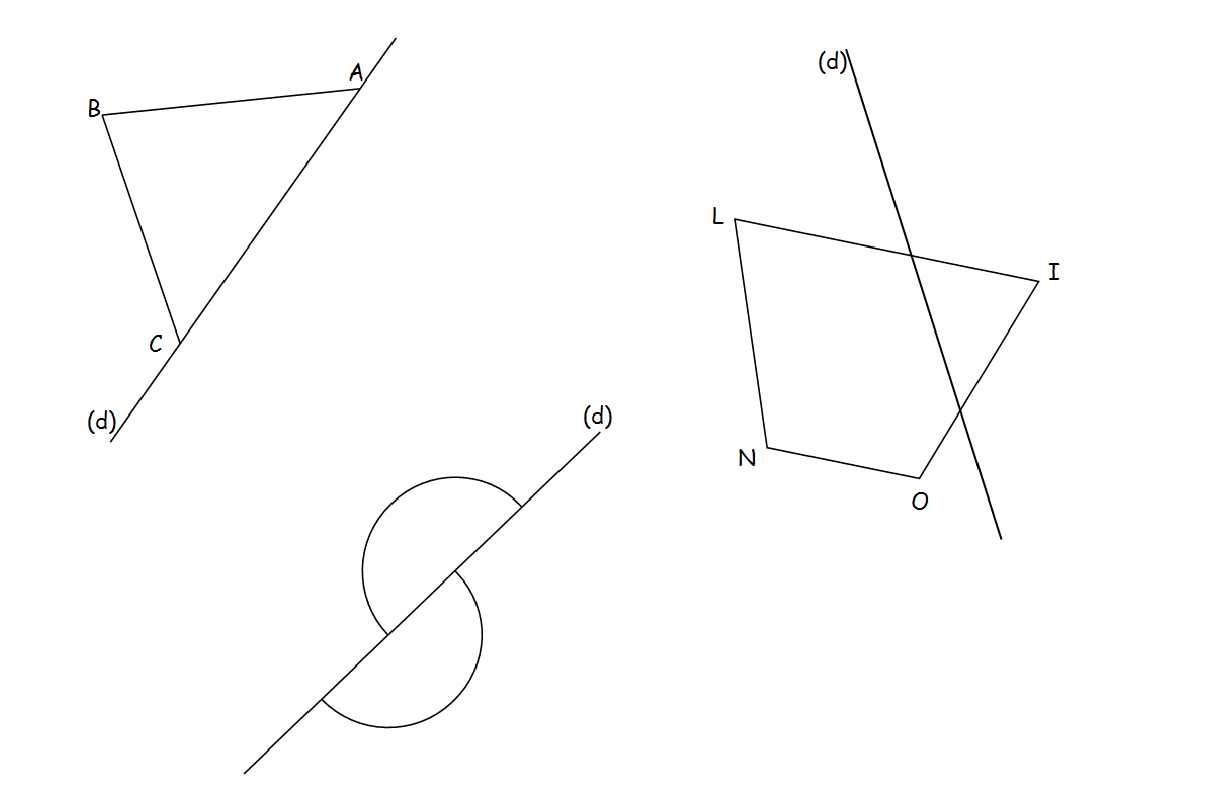
\includegraphics[scale=0.5]{exo1.eps} 
 \end{center}
 
 \initq \q Exprimer son périmètre, en mètre, en fonction de $x$.\\
 
 \q Quelles sont les dimensions de ce rectangle quand son périmètre est égal à 31 m ?\\
 
 \vspace*{0.5cm}
 
 \exo
 
 Trouve un nombre sachant que son triple augmenté de 2 est égal à son double augmenté de 3.\\

\vspace*{0.5cm}

\exo\\

Noah veut acheter des livres qui coûtent le même prix.\\
S'il en achète 7, il lui manque 1,20 euros. S'il en achète 6, il lui reste 3,50 euros.\\

Quel est le prix d'un livre ?\\
\vspace*{0.5cm}

\exo \\

Deux frères, Marc et Jean, possèdent chacun un jardin. L'aire du jardin de Marc vaut les $\dfrac{3}{4}$ de l'aire du jardin de Jean. Les deux frères possèdent en tout 1 470 $ m^{2} $.\\

Quelles sont les aires des jardins de Marc et de Jean  ?\\





 
 \vspace*{0.5cm}
 
 \exo

Thomas a obtenu 11 et 16 aux deux premiers contrôles de Maths.\\
Quelle note doit-il avoir au troisième contrôle pour obtenir 15 de moyenne ?\\

\vspace*{0.5cm}
 
 


\exo



\bmul{2}

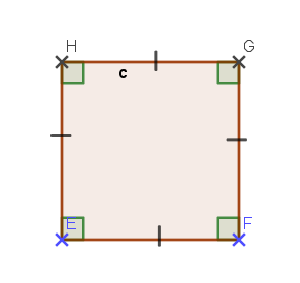
\includegraphics[scale=0.75]{carre.eps} 

\columnbreak
\initq 
\begin{flushleft}
\q Exprimer l'aire du rectangle AMNP en fonction de $x$.


\q Trouver x pour que l'aire de AMNP soit égale au tiers de l'aire du carré ABCD.\\
\end{flushleft}



\emul



\vspace*{0.5cm}

\exo
 
 Justine a 8 ans et sa grand-mère a 50 ans. \\
Dans combien d'années, l'âge de sa grand-mère sera le triple de celui de Justine ?\\

\vspace*{0.5cm}

\exo 

 Une brique pèse 1 kg plus la moitié de son poids.      Combien pèse-t-elle ?
\vspace*{0.5cm}



\end{document}
